% Created 2017-11-13 Mon 12:07
% Intended LaTeX compiler: pdflatex
\documentclass[11pt]{article}
\usepackage[utf8]{inputenc}
\usepackage[T1]{fontenc}
\usepackage{graphicx}
\usepackage{grffile}
\usepackage{longtable}
\usepackage{wrapfig}
\usepackage{rotating}
\usepackage[normalem]{ulem}
\usepackage{amsmath}
\usepackage{textcomp}
\usepackage{amssymb}
\usepackage{capt-of}
\usepackage{hyperref}
\usepackage[margin=.75in]{geometry}
\author{Anthony Tam}
\date{\today}
\title{CSC373, Fall 2017}
\hypersetup{
 pdfauthor={Anthony Tam},
 pdftitle={CSC373, Fall 2017},
 pdfkeywords={},
 pdfsubject={},
 pdfcreator={Emacs 26.0.50 (Org mode 9.0.9)}, 
 pdflang={English}}
\begin{document}

\maketitle

\section*{Lecture One}
\label{sec:org337b1ad}
\subsection*{Administrative}
\label{sec:orga749f19}
\begin{itemize}
\item Vincent Maccio
\item vincent.maccio@utoronto.ca
\item vincentmaccio.com
\item Office Hours
\begin{itemize}
\item DH3015
\item 11:00 to 12:00
\item 1:00 to 2:00
\end{itemize}
\item Email subject
\begin{itemize}
\item CSC373 - \{Your Name\}
\end{itemize}
\end{itemize}
\subsection*{Introduction to Big Oh}
\label{sec:org87e2215}
\begin{itemize}
\item f(n) = O(g(n))
\begin{itemize}
\item g(n) bounds f(n) from above by some constant factor\ldots{} evantually.
\item Formally, f(n) = O(g(n)) \(\leftrightarrow\) \(\exists\)c, n\(_{\text{o}}\):\(\forall\) n\textgreater{}n\(_{\text{o}}\), f(n)\(\le\)cg(n)
\end{itemize}
\item Prove 20n\(^{\text{2}}\)+4n-8 = O(n\(^{\text{2}}\))
\begin{itemize}
\item find c, n\(_{\text{o}}\), f(n) \(\le\) cg(n) \(\forall\) n>n\(_{\text{o}}\)
\item c = 24, n\(_{\text{o}}\) = 1
\item f(n) \(\le\) 20n\(^{\text{2}}\) + 4n\(^{\text{2}}\) for n>1
\item f(n) \(\le\) 24n\(^{\text{2}}\) \(\le\) 24g(n)
\end{itemize}
\item Prove n\(^{\text{3}}\) \(\ne\) O(n\(^{\text{2}}\))
\begin{itemize}
\item Assume: n\(^{\text{3}}\) \(\le\) cn\(^{\text{2}}\), \(\forall\)n>n\(_{\text{o}}\)
\item \(\forall\) n > 1, n\(^{\text{3}}\) \(\le\) 10000n\(^{\text{2}}\), n>c, n\(^{\text{3}}\)>cn\(^{\text{2}}\) consider n>c
\end{itemize}
\item Prove or Disprove: 2\(^{\text{2n}}\) = O(2\(^{\text{n}}\) + n\(^{\text{2}}\))
\begin{itemize}
\item If g(n)=O(g'(n)) and f(n)\(\ne\)O(g'(n)) then, f(n)\(\ne\)O(g(n))
\item Let g'(n)=2\(^{\text{n}}\), g(n)=2\(^{\text{n}}\)+n\(^{\text{2}}\), can we show g(n)=O(g'(n)), then 2\(^{\text{2n}}\) \(\ne\) O(2\(^{\text{n}}\))
\item 2\(^{\text{n}}\) + n\(^{\text{2}}\) = O(n\(^{\text{n}}\))
\item n\(_{\text{o}}\) \(\ge\) 4, 2\(^{\text{n}}\)+n\(^{\text{2}}\) \(\ge\) 22\(^{\text{n}}\) = O(2\(^{\text{n}}\))
\item f(n)\(\ne\)O(g(n)) \(\leftarrow\) \(\forall\)c, \(\exists\)n': \(\forall\)n>n': f(n)>cg(n)
\item 2\(^{\text{2n}}\) \(\ne\) O(2\(^{\text{n}}\))\ldots{}. 2\(^{\text{2n}}\) = 2\(^{\text{n}}\) \(\cdot\) 2\(^{\text{n}}\)\ldots{}. 2\(^{\text{n}}\) \(\cdot\) 2\(^{\text{n}}\) \(\le\) c2\(^{\text{n}}\) \(\rightarrow\) 2\(^{\text{n}}\) \(\le\) c
\item let n+1=log\(_{\text{2}}\)(c) \(\therefore\)Contradiction, QED.
\end{itemize}
\item If f\(_{\text{1}}\)(n) = O(g\(_{\text{1}}\)(n)) and f\(_{\text{2}}\)(n) = O(g\(_{\text{2}}\)(n)), prove max(f\(_{\text{1}}\)(n), f\(_{\text{2}}\)(n)) = O(max(g\(_{\text{1}}\)(n), g\(_{\text{2}}\)(n)))
\begin{itemize}
\item let c\(_{\text{1}}\), n\(_{\text{o1}}\) be valid values to prove f\(_{\text{1}}\)(n) = O(g\(_{\text{1}}\)(n))
\item let c\(_{\text{2}}\), n\(_{\text{o2}}\) be valid values to prove f\(_{\text{2}}\)(n) = O(g\(_{\text{2}}\)(n))
\item let c=max(c\(_{\text{1}}\), c\(_{\text{2}}\)) and n\(_{\text{o}}\)=max(n\(_{\text{o1}}\), n\(_{\text{o2}}\))
\item n'\(\ge\)n\(_{\text{o}}\), consider the case where f\(_{\text{1}}\)(n') \(\ge\) f\(_{\text{2}}\)(n')
\begin{itemize}
\item f\(_{\text{1}}\)(n') \(\le\) c\(_{\text{1}}\) g\(_{\text{1}}\)(n') \(\le\) max(c\(_{\text{1}}\), c\(_{\text{2}}\))max(g\(_{\text{1}}\)(n'), g\(_{\text{2}}\)(n'))
\end{itemize}
\item Prove the other directional by repeating the above step
\end{itemize}
\end{itemize}
\section*{Lecture Two}
\label{sec:org2cdd144}
\subsection*{Greedy}
\label{sec:org727d557}
\begin{itemize}
\item What's good now (local) vs what's good later (global)
\item Define some rule/metric/heuristic
\item Do what's best for that rule
\end{itemize}
\subsubsection*{Advantages}
\label{sec:org9bacdb2}
\begin{itemize}
\item Easy to think of
\item Easy to implement
\end{itemize}
\subsubsection*{Disadvantages}
\label{sec:org03bb863}
\begin{itemize}
\item Proving it's optimal vs suboptimal
\end{itemize}
\subsubsection*{Knapsack Problem}
\label{sec:org201d22e}
\begin{itemize}
\item You're given a set of items, S, and a maximum capacity C
\item s \(\in\) S has an assosiated weight and calue (W\(_{\text{s}}\), V\(_{\text{s}}\))
\item max total value S'\(\subset\) S, such total weight of S' is \(\le\) C
\end{itemize}
\begin{itemize}
\item Solutions
\label{sec:org5dbef75}
\begin{itemize}
\item Brute Force: O(2\(^{\text{n}}\))
\item Take highest value
\item Lowest Weight
\item Highest value per weight
\item \textbf{There is no polynomial solution for this}
\end{itemize}
\end{itemize}
\subsubsection*{Scheduling Jobs}
\label{sec:org484e496}
\begin{itemize}
\item Given a set of jobs (n of them)
\item Each job, i, has a start time, s(i), and a finish time, f(i)
\item Schedule the maximum \# of jobs which don't conflict
\end{itemize}
\begin{itemize}
\item Solutions
\label{sec:org62de941}
\begin{itemize}
\item Brute Force: O(2\(^{\text{n}}\))
\item Take the shortest job
\item Take the earliest start time
\item Take the earliest finish time
\begin{itemize}
\item Assume A* is an optimal solution
\item Assume A\(^{\text{G}}\) is the schedule returned by the earliest finish time algorithm (EFT)
\item Let A*i: i\(_{\text{1}}\), \ldots{}, i\(_{\text{m}}\) A\(^{\text{G}}\): j\(_{\text{1}}\), \ldots{}, j\(_{\text{k}}\)
\item We need to show k=m 
\begin{itemize}
\item f(i\(_{\text{r - 1}}\)) \(\le\) f(i\(_{\text{r}}\))
\item f(j\(_{\text{r - 1}}\)) \(\le\) f(j\(_{\text{r}}\))
\end{itemize}
\item Lemma: \(\forall\)r\(\le\)k, f(j\(_{\text{r}}\)) \(\le\) f(i\(_{\text{r}}\))
\begin{itemize}
\item Prove via induction
\begin{itemize}
\item Need to show f(j\(_{\text{i}}\)) \(\le\) f(i\(_{\text{i}}\)), from EFT f(j) \(\le\) f(i) \(\forall\) i \(\rightarrow\) f(j\(_{\text{i}}\)) \(\le\) f(i\(_{\text{i}}\))
\item Assume f(j\(_{\text{r - 1}}\)) \(\le\) f(i\(_{\text{r - 1}}\))
\item Show f(j\(_{\text{r}}\)) \(\le\) f(i\(_{\text{r}}\)), relate f(i\(_{\text{r - 1}}\)) to s(i\(_{\text{r}}\))
\begin{itemize}
\item f(i\(_{\text{r - 1}}\)) \(\le\) s(i\(_{\text{r}}\)), jobs don't conflict
\item Case 1: A\(^{\text{G}}\) chooses the same job as A* (at the r\(^{\text{th}}\) index)
\begin{itemize}
\item For free we know f(j\(_{\text{r}}\)) \(\le\) f(i\(_{\text{r}}\))
\end{itemize}
\item Case 2: A\(^{\text{G}}\) chooses a different job, from the greedy rule
\begin{itemize}
\item f(j\(_{\text{r}}\)) \(\le\) f(i\(_{\text{r}}\))
\end{itemize}
\end{itemize}
\end{itemize}
\end{itemize}
\item Assume A\(^{\text{G}}\) is not optimal, m \textgreater{} k
\begin{itemize}
\item \(\therefore\) in A* there is a job which starts after i\(_{\text{k}}\) \(\rightarrow\) s(i\(_{\text{k+1}}\)) \(\ge\) f(i\(_{\text{k}}\)) \(\ge\) f(j\(_{\text{k}}\))
\begin{itemize}
\item Contradiction, A\(^{\text{G}}\) would have at least choosen i\(_{\text{k + 1}}\)
\item \(\therefore\) A\(^{\text{G}}\) is optimal
\end{itemize}
\end{itemize}
\item "Stays Ahead" proof
\begin{verbatim}
def Schedule(J):
   #Sort J bu finish time
   S = { }
   s = S + J[1]
   last_added = J[1]
   for i=2 to n:
      if J[i].start_time > last_added.finish_time:
         S = S + J[i]
         last_added = J[i]
   return S
\end{verbatim}
\end{itemize}
\item Job with the least conflicts
\item Job with the most conflicts
\end{itemize}
\end{itemize}
\section*{Lecture Three}
\label{sec:orgd2696f5}
\subsection*{Greedy}
\label{sec:orga86788b}
\begin{itemize}
\item Single Source Shortest
\end{itemize}
\subsubsection*{What is a graph?}
\label{sec:org402f63e}
\begin{itemize}
\item G=(V, E)
\begin{itemize}
\item V is the set of verticies
\item E is the set of edges
\item E \(\subset\) VxV e=(u, v)
\item |E| \(\le\) |V|\(^{\text{2}}\)
\item weight function w(), w(e) \(\triangleq\) the wright of edge e
\end{itemize}
\end{itemize}
\subsubsection*{MST, what is it? G=(V, E)}
\label{sec:orge515fec}
\begin{itemize}
\item It's a connected graph (V, T)
\item The weight of all edges is minimized
\item min \(\sum_{\text{e}\in\text{t}}\) w(e), |T|=n - 1, n=|V|
\end{itemize}
\begin{itemize}
\item Kruscals
\label{sec:org2550319}
\begin{verbatim}
def kruscals(V, E):
    #Sort E by nondecending order by w(e)
    T = {}
    for i in range (1, |E|):
        (e, v) = e[i]
        if u is not connected to v in T:
            T = T + {e[i]}
\end{verbatim}
\begin{itemize}
\item T\(^{\text{K}}\): is the spanning tree returned by Kruscal's algorithm
\item T*: is the minimum spanning tree
\item T\(^{\text{K}}_{\text{1}}\): T\(^{\text{K}}\) after the i\(^{\text{th}}\) iteration of Kruscal's
\item Show \(\forall\) i, \(\exists\) a MST which agrees with T\(_{\text{i}}\), for frst i choices
\begin{itemize}
\item Base Case: i=0, T\(^{\text{K}}_{\text{i}}\) = \{\}
\item Assume exists an MST T\(^{\text{*}}\) that agrees with T\(^{\text{K}}_{\text{i-1}}\)
\item Show this for i
\begin{itemize}
\item Consider the edge e\(_{\text{i}}\)
\begin{center}
\begin{tabular}{rlll}
Case & T\(_{\text{i}}^{\text{k}}\) & T\(^{\text{*}}\) & Is Trivial?\\
\hline
1 & exclude & exclude & Yes\\
2 & exclude & include & No\\
3 & include & exclude & No\\
4 & include & include & Yes\\
\end{tabular}
\end{center}
\item Looking more into case 2 (Kruscal excluded, OPT included)
\begin{itemize}
\item If T\(^{\text{*}}\) includes e\(_{\text{i}}\), it creates a cycle
\begin{itemize}
\item However, MSTs don't have cycles, \(\Rightarrow \Leftarrow\)
\end{itemize}
\end{itemize}
\item Case 3 (Kruscal included, OPT excluded)
\begin{itemize}
\item let e\(_{\text{i}}\)=(v, u)
\item At this point, u and v are not connected
\begin{itemize}
\item There must be an edge e\(_{\text{j}}\) that will connect u and v (potentially be indirectly)
\item If we can show e(e\(_{\text{max}}\))\(\le\)w(e\(_{\text{i}}\)), w(e\(_{\text{max}}\))\(\ge\)w(e\(_{\text{j}}\))\(\ge\)w(e\(_{\text{i}}\))
\item Remove e\(_{\text{j}}\), new T' has total weight \(\le\) w(T\(^{\text{*}}\)), but ut includeds e\(_{\text{i}}\)
\end{itemize}
\end{itemize}
\end{itemize}
\end{itemize}
\end{itemize}
\begin{center}
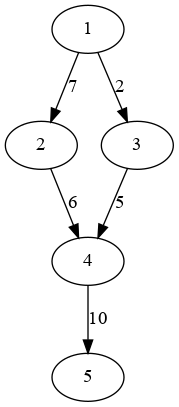
\includegraphics[width=.9\linewidth]{kruscals.png}
\end{center}
\end{itemize}
\subsubsection*{Dijkstra's Algorithm}
\label{sec:orgb528f62}
\begin{itemize}
\item Single source
\item All edge weights are positive
\end{itemize}
\begin{verbatim}
def Dijkstra(V, E):
  S = {} #Set of visited verticies
  for v in V:
    d[v] = 999 #Some large number
  d[source] = 0
  while v not in x:
    v = non_visited_vertex with the smallest d[v]
    for all edges:
      if u is not in s and d[v] + w(v, u) < d[u]:
        d[u] = d[v] + w(u, v)
    S = S + {v}
\end{verbatim}

\begin{center}
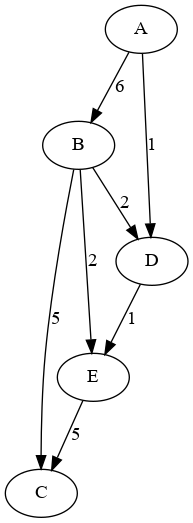
\includegraphics[width=.9\linewidth]{dijkstra.png}
\end{center}
\begin{center}
\begin{tabular}{llll}
Vertex & d[v] & Pred & Visited\\
\hline
A & 0 & None & Yes (1)\\
B & \(\infty\) -> 6 -> 3 & None -> A -> D & Yes (4)\\
C & \(\infty\) -> 7 & None -> E & Yes (5)\\
D & \(\infty\) -> 1 & None -> A & Yes (2)\\
E & \(\infty\) -> 2 & None -> D & Yes (3)\\
\end{tabular}
\end{center}
\begin{itemize}
\item What do we need from the algo? All in O(log(n))
\begin{itemize}
\item getMin()
\item updateKey(v, n)
\item deleteMin()
\end{itemize}
\item Show when you visit d[u], d[u] is the shortest distance in all visited nodes
\begin{itemize}
\item d[y] \(\le\) d[u] cannot be shorter but getting a node which is outside the currently viisted nodes
\end{itemize}
\end{itemize}
\section*{Lecture Four}
\label{sec:org6e20005}
\subsection*{Dynamic Programming}
\label{sec:orgd3f1ef1}
\begin{enumerate}
\item Define the overall problem as a set of subproblems
\item Relate these subproblems to eachother
\item Solve ans SAVE subproblems
\begin{itemize}
\item Easier to understand
\item Decreases complexity
\end{itemize}
\end{enumerate}
\subsubsection*{Longest Common Subsequence}
\label{sec:org515317b}
\begin{itemize}
\item Given 2 strings X and Y a common subsequence is a string of characters s such that the order of the characters in s appear in X and Y in the same order
\begin{itemize}
\item X = xxadbxxxc, Y = abyydyc, substring = "ab", subsequence = "abc" or "adc"
\end{itemize}
\item If X is length n, how many subsequences does it contain
\begin{itemize}
\item 2\(^{\text{n}}\), resulting in O(2\(^{\text{n + m}}\)) where n = len(X) and m = len(Y)
\end{itemize}
\item LCS(X\(_{\text{i}}\), Y\(_{\text{j}}\)) \(\Rightarrow\) the largest common subsequence of X[:i] and Y[:j]
\begin{itemize}
\item This will lead to LCS(X\(_{\text{n}}\), Y\(_{\text{m}}\)), the entire problem
\end{itemize}
\[ \begin{cases} 
        1 + LCS(X_{i - 1}) & X[i] = Y[j]\\
        max(LCS(X_i, Y_{j - 1}), LCS(X_{i - 1}, Y_j)) & X[i] \ne Y[j]
        \end{cases}
      \]
\end{itemize}
\begin{verbatim}
def LCS(X, Y):
  n = len(X)
  m = len(Y)
  SP = int[n, m]
  for i in range (1, n):
      for j in range (1, m):
        if X[i] == Y[j]:
          SP[i][j] = SP[i-1][j-1] + 1
        else:
          SP[i][j] = max(SP[i-1][j], SP[i][j-1])
  return SP[n][m]
\end{verbatim}
\begin{itemize}
\item Example
\label{sec:org1c86c5d}
\begin{itemize}
\item X = "AGGTAB", Y = "GTUAYB"
\end{itemize}
\begin{center}
\begin{tabular}{rrrrrrrr}
\(\frac{Y}{X}\) & 0 & 1 & 2 & 3 & 4 & 5 & 6\\
\hline
0 & 0 & 0 & 0 & 0 & 0 & 0 & 0\\
1 & 0 & 0 & 0 & 0 & 1 & 1 & 1\\
2 & 0 & 1 & 1 & 1 & 1 & 1 & 1\\
3 & 0 & 1 & 1 & 1 & 1 & 1 & 1\\
4 & 0 & 1 & 2 & 2 & 2 & 2 & 2\\
5 & 0 & 1 & 2 & 3 & 3 & 3 & 3\\
6 & 0 & 1 & 2 & 2 & 3 & 3 & 4\\
\end{tabular}
\end{center}
\end{itemize}

\subsubsection*{Knapsack Problem}
\label{sec:orge06c867}
\begin{itemize}
\item Assume the capacity, all weights, and all values are all ints
\item Subproblem: K(i, c) \(\triangleq\) optimal value when using only the first i items with capacity c
\item Base case: k(0, c) = 0 and k(i, 0) = 0
\[ \begin{cases} 
        K(i - 1, c) & c < w_i\\
        max(K(i - 1, c - w_i) + v_i, K(i -1, c)) & c \ge w_i
        \end{cases}
      \]
\begin{itemize}
\item Note, case 2 is the max of including or excluding
\end{itemize}
\end{itemize}
\begin{itemize}
\item Example
\label{sec:orgcb7cfd8}
\begin{itemize}
\item C = 10
\end{itemize}
\begin{center}
\begin{tabular}{rrr}
Item & Weight & Value\\
\hline
1 & 1 & 2\\
2 & 2 & 3\\
3 & 6 & 6\\
4 & 8 & 9\\
\end{tabular}
\end{center}
\begin{itemize}
\item After running:
\end{itemize}
\begin{center}
\begin{tabular}{rrrrrrrrrrrr}
\$\frac{C}{Items} & 0 & 1 & 2 & 3 & 4 & 5 & 6 & 7 & 8 & 9 & 10\\
\hline
0 & 0 & 0 & 0 & 0 & 0 & 0 & 0 & 0 & 0 & 0 & 0\\
1 & 0 & 2 & 2 & 2 & 2 & 2 & 2 & 2 & 2 & 2 & 2\\
2 & 0 & 2 & 3 & 5 & 5 & 5 & 5 & 5 & 5 & 5 & 5\\
3 & 0 & 2 & 3 & 5 & 5 & 5 & 6 & 8 & 9 & 11 & 11\\
4 & 0 & 2 & 3 & 5 & 5 & 5 & 6 & 8 & 9 & 11 & 12\\
\end{tabular}
\end{center}
\begin{itemize}
\item O(nc), psudo-polynomial
\end{itemize}
\end{itemize}
\section*{Lecture Five}
\label{sec:orgfd212fa}
\subsection*{Midterm}
\label{sec:org783bc03}
\begin{itemize}
\item Next week, Oct 23\(^{\text{rd}}\)
\item 11:00am - 1:00pm
\end{itemize}
\subsection*{Shortest Path}
\label{sec:orga7fd871}
\subsubsection*{Dijkstra's Algorithm}
\label{sec:orge26d1e2}
\begin{itemize}
\item Source S, find \(\forall\)v sp(s, v)
\begin{itemize}
\item O(V\(^{\text{2}}\) log V) (priority heap)
\item O(E r V log C) (fib heap)
\end{itemize}
\item What about \(\forall\)u,v sp(u, v)
\begin{itemize}
\item O(EV + V\(^{\text{2}}\) log V)
\end{itemize}
\item Run Dijkstra from every node
\begin{itemize}
\item V - 1 \(\le\) E \(\le\) V\(^{\text{2}}\)
\item E = \(\theta\)(V\(^{\text{2}}\)) \(\Rightarrow\) G is dence
\begin{itemize}
\item O(V\(^{\text{3}}\))
\end{itemize}
\item E = \(\theta\)(V) \(\Rightarrow\) G is sparse
\begin{itemize}
\item O(V\(^{\text{2}}\) log V)
\end{itemize}
\end{itemize}
\item No negative weights
\end{itemize}
\subsubsection*{Bellman-Ford}
\label{sec:org2f385ad}
\begin{itemize}
\item Single Source
\item Allows negative weights
\item Worse case runtime: O(V\(^{\text{3}}\))
\begin{itemize}
\item For all pairs shortest path: O(V\(^{\text{4}}\))
\end{itemize}
\end{itemize}
\subsubsection*{Floyd-Warshall}
\label{sec:org0b973a9}
\begin{itemize}
\item Dynamic programming
\item All pairs
\item Define the sub problems
\begin{itemize}
\item We want SP(i, j)
\item SP(i, j, k) \(\triangleq\) the shortest path from i to j when I have access to the first k nodes, plus i and j
\item SP(i, j) = SP(i, j, n) where n = |V|
\item SP(i, j, k) = SP(i, j, k - 1) if the shortest path between i and k given access to the first k nodes doesn't include node k
\item SP(i, j, k) = SP(i, j, k) + SP(k, j, k) if the k\(^{\text{th}}\) node is used
\begin{itemize}
\item SP(i, j, k) = min(SP(i, j, k-1), SP(i, k, k - 1) + SP(k, j, k - 1)) is a simplified problem which suits DP
\end{itemize}
\item SP(i, i, 0) = 0
\end{itemize}
\[
        SP(i, j, 0) = \begin{cases} 
          w(i, j) & (i, j)\in{}E \\
          \infin \\
        \end{cases}
      \]
\begin{verbatim}
def Floyd(G = (V, E)):
  for v in V:
    d[v][v][0]= 0
  for node(u, v) in E:
    d[u][v][0] = W(u, v)
  for k in range(1, len(V)):
    for i in range(1, len(V)):
      for j in range(1, len(V)):
        if d[i][j][k-1] > d[i][j][k-1] + d[k][j][k-1]:
          d[i][j][k] = d[i][k][k-1] + d[k][j][k-1]
        else:
          d[i][j][k] = d[i][j][k-1]
\end{verbatim}
\end{itemize}
\subsection*{More DP Problems}
\label{sec:orga638b01}
\begin{itemize}
\item Can a string s be split into words
\begin{itemize}
\item canSplit("abcnmcdms") \(\rightarrow\) False
\item canSplit("ilikeoranges") \(\rightarrow\) True
\end{itemize}
\item String s has length of n
\item SP(s\(_{\text{i}}\))
\begin{itemize}
\item let s\(_{\text{i}}\) denote the first i characters of s
\item let s[i, j] be the substring of s from s[i] to s[j] inclusive \(\Rightarrow\) s[i, i] = s[i]
\item canSplit(s\(_{\text{i}}\)) = V\(^{\text{i}}_{\text{j=1}}\)(canSplit(s\(_{\text{j-1}}\)\(_\)) \^{} isWord(s[j, i]))
\end{itemize}
\end{itemize}
\section*{Lecture Six}
\label{sec:org2d5b31c}
\subsection*{Flow Network}
\label{sec:org858a7fc}
\begin{itemize}
\item Directed Graph, G=(V, E)
\item A single source vertex s
\item A single target vertex t
\item if (u, v)\(\in\)E \(\Rightarrow\) (v, u)\(\notin\)E: no anti-parallel edge
\item Non-negative capacity function, c(u, v)
\end{itemize}
\subsubsection*{Def'n}
\label{sec:org33e0cef}
\begin{itemize}
\item Let f(u, v) be a "flow" value for each edge (u, v)
\item f is a valid flow if it satisfies two properties
\begin{enumerate}
\item \(\forall\)u, v O\(\le\)f(u, v)\(\le\)c(u, v)
\item \(\forall\)u \(\in\) V-\{s, t\} \(\sum_{\text{v }\in\ \text{V}}\)f(v, u) = \(\sum_{\text{v }\in\ \text{V}}\)f(u, v)
\end{enumerate}
\end{itemize}
\subsubsection*{First Idea}
\label{sec:orge5222cd}
\begin{itemize}
\item Keep finding valid paths from s to t, send as much flow as possible, keep repeating this until no path remains
\begin{itemize}
\item Return |f|
\item Find a new path and send low, called augmenting path
\item Informally, Ford-Fulkerson Method
\end{itemize}
\end{itemize}
\subsection*{Max-flow-Min-cut}
\label{sec:org07705ac}
\begin{itemize}
\item FF is correct iff
\begin{enumerate}
\item |f| is a max flow \(\Rightarrow\) \(\exists\) an augmenting path in G\(_{\text{f}}\)
\item if ther's no augmenting path in G\(_{\text{f}}\) \(\Rightarrow\) |f| is maximized
\end{enumerate}
\end{itemize}
\subsubsection*{Def'n}
\label{sec:org421b8a8}
\begin{itemize}
\item A cut (S, T) of a flow netowkr G=(V, E) is a partition of V such that s\(\in\)S, t\(\in\)T, S\union{}T = V
\item Flow across a cut (S, T) = \(\sum_{\text{u }\in\ \text{S}}\) \(\sum_{\text{v }\in\ \text{T}}\) f(u, v) - \(\sum_{\text{u }\in\ \text{S}}\) \(\sum_{\text{v }\in\ \text{T}}\) f(v, u)
\end{itemize}
\section*{Lecture Seven}
\label{sec:org046f8d9}
\subsection*{Recap}
\label{sec:org09554cc}
\begin{itemize}
\item Given a directed graph or a flow network, what's the max flow form from s to t
\begin{itemize}
\item Find a path from s to t
\item Send flow across path
\item Doesn't work
\end{itemize}
\item Have a correspinding residual netowkr
\begin{itemize}
\item Keeps track of backflows
\item Find "augmenting paths" in the RN and send flow
\item Repeat
\item This works vis max flow main-cut theorem
\begin{itemize}
\item Ford-Fulkerson method
\end{itemize}
\item Let f* denote max flow; m \# of edges
\item O(m) we can find a path, update flows, capacities, etc)
\begin{itemize}
\item Psuedopolynomial
\end{itemize}
\end{itemize}
\end{itemize}
\subsection*{Max Flow}
\label{sec:orge81cefc}
\begin{itemize}
\item When finding paths, use BFS
\begin{itemize}
\item We complexity O(nm\(^{\text{2}}\)) = O(VE\(^{\text{2}}\))
\item This is called Edmond-Karp's algorithm
\end{itemize}
\end{itemize}
\subsubsection*{Maximum-Matching in bipartite graphs}
\label{sec:orga14c08d}
\begin{itemize}
\item Given a graph G=(V, E) and two disjoint sets L and R, where L\(\cup\)R = V and all edges "start" in L and "end" in R
\begin{itemize}
\item Find M\subseteq{}E where \(\forall\)(u, v)\(\in\) M, u and v appear only once
\end{itemize}
\end{itemize}
\section*{Lecture Eight}
\label{sec:org8f7a5b6}
\subsection*{Complexity}
\label{sec:org1df95b6}
\subsubsection*{P - Polynomial Time}
\label{sec:org2586ddd}
\begin{itemize}
\item All problems which can be solved in polynomial time O(n\(^{\text{k}}\))
\begin{itemize}
\item Sorting, searching, graph problems, max-flow
\item Knapsack is not in P
\end{itemize}
\item Considered "easy"
\end{itemize}
\subsubsection*{NP - Non-deterministic Polynomial Time}
\label{sec:org14c3b2a}
\begin{itemize}
\item We can determine if a given solution is correct or not in polynomial time
\item Considered "hard"
\item Sudoku
\begin{itemize}
\item Fill in the grid so the digits 1-9 appear exactly once in every row, column, and subgrid (3x3 square)
\end{itemize}
\item Knapsack Problem-Decision
\begin{itemize}
\item Given a knapsack problem, does there exist a solution which has total value of at least V
\item What is someome gives you a set of items and claims it's a solution
\begin{itemize}
\item Sum the values (\(\sum\)v\(_{\text{i}}\) \(\ge\) V)
\item Check total weight (\(\sum\)w\(_{\text{i}}\) \(\le\) C)
\end{itemize}
\end{itemize}
\item Can check in polynomial time
\item P\(\subset\)NP
\end{itemize}
\begin{itemize}
\item NP-Complete
\label{sec:org5017125}
\begin{itemize}
\item The "hardest" problems to solve in NP
\item If you solve these, you solve all NP problems
\end{itemize}
\item NP-Hard
\label{sec:org1a3097b}
\begin{itemize}
\item All problems which are just as "hard" as the NP complete problems
\end{itemize}
\end{itemize}
\subsubsection*{What do you need to solve an NP problem}
\label{sec:orgfaffd1b}
\begin{itemize}
\item Sacrifice Generality
\begin{itemize}
\item Knapsack on A1
\end{itemize}
\item Sacrifice Optimality
\begin{itemize}
\item Approximation, within a constant factor of the optimal
\end{itemize}
\item Sacrifice Reliability
\begin{itemize}
\item Get the optimal solution most of the time
\end{itemize}
\item Solve P = NP
\end{itemize}
\subsection*{Vertex Cover Problem}
\label{sec:org25e5b16}
\begin{itemize}
\item Given a graph G=(V, E) a subset of verticies C\subseteq{}V us a vertex cover iff \(\forall\)(u, v)\(\in\)E: u\(\in\)C or v\(\in\)C
\item Finding if there exists a vertex cover of size |C|=k is NP-Complete
\item Finding the smallest vertex cover, min(|C|) is NP-Hard
\end{itemize}
\begin{verbatim}
def greedy_sol():
    G = {}
    E_prime = {}
    while E_prime is not {}:
      u, v = some_edge_in(E_prime)
      C = C + {u, v}
      remove_all_incident_edges((u, v))
    return C
\end{verbatim}
\end{document}
